\documentclass[manuscript,screen,review]{acmart}
\usepackage[T1]{fontenc}
\usepackage{tabularx}
\usepackage{listings}
\setcopyright{none}
\settopmatter{printacmref=false}
\renewcommand\footnotetextcopyrightpermission[1]{}
\acmDOI{}
\acmISBN{}
\acmYear{}
\acmConference[]{}{}{}
\title{Wide Leaf Filtering for Exact Ternary Subset Sum Root Reporting}
\author{Naman PM}
\renewcommand{\shortauthors}{Naman PM}
\begin{document}
\begin{abstract}
Representation algorithms for random Subset Sum generate large lists of signed vectors and repeatedly join them under modular constraints. At the final ternary merge, a short arithmetic projection can admit a large number of candidates even when the full relation has no solutions. We study exact arithmetic root reporting with inexpensive rejection ahead of candidate recovery. The Adaptive Radix Wide-Leaf Filter (ARWLF) partitions residual keys into fixed thirteen-bit leaves, routes source pairs with explicit carries, and tests byte occupancy in the target leaf. An AVX2 implementation evaluates one source entry against sixteen entries at a time; surviving pairs undergo full quotient comparison and original-residue verification. On an Intel Core Ultra 9 275HX, ARWLF achieves geometric-mean speedups of 53.1 over the tiled baseline on fourteen calibration microproblems and 52.9 on fifteen microproblems from three holdout roots at dimension 108. Against a baseline that already rejects full-width mismatches before the shared output sink, the corresponding gains are 32.8 and 32.4. Controlled source and target thinning identify both the occupancy crossover and the contribution of candidate suppression. Sparse dimension-72 roots favor a different reporter. A complete prepared dimension-108 root with one constructed positive target takes 59.6 minutes in one ARWLF pass. The method preserves exact arithmetic reporting and entry multiplicity; production binary-root certification remains separate. Its contribution is a finite-size improvement in pair-processing cost, with no change to the asymptotic Subset Sum exponent.
\end{abstract}
\ccsdesc[500]{Theory of computation~Design and analysis of algorithms}
\keywords{Subset Sum; ternary representations; experimental algorithmics; modular joins; SIMD; exact filtering}
\maketitle
\raggedbottom
\section{Introduction}
The complexity of a representation algorithm is determined by more than the sizes of its final lists. Intermediate arithmetic matches must be discovered, checked for coordinate compatibility, and recovered as original entries. A merge that is cheap in terms of accepted parents can therefore be expensive on the machine: a short projection may generate many candidates, and nearly all of them can fail the remaining conditions. This distinction has appeared in the analysis of representation methods themselves. Becker, Coron, and Joux explicitly account for the intermediate list before filtering, rather than charging only the final filtered list \cite{bcj2011}. It also creates a practical optimization question: when many inexpensive pair tests are unavoidable, how much work should accompany each test?

This paper addresses that question at the final ternary root merge of a classical Ternary Representation Technique (TER) construction. Li's depth-three algorithm forms eighteen logical level-three lists, then nine level-two lists, three level-one lists, and a final root list \cite{li2025}. The root arithmetic is a modular three-list reporting problem. Its large source families admit billions of logical pairs per family cell at the evaluated dimension. Testing every pair with an expensive membership operation, or recovering every match of a short projection before checking the remaining bits, places the cost in the wrong part of the computation.

The Adaptive Radix Wide-Leaf Filter changes this cost distribution. Low residual bits route a pair to exactly one target leaf. Independent occupancy maps for the next bytes reject a pair whenever a required byte is absent. The maps are deliberately weaker than full equality: they summarize target bytes without retaining their correlations. That loss of information is useful because a small, register-friendly test can reject most pairs before original entry identities or wide residues are processed. Exact comparison remains on the survivor path.

The central implementation choice is to organize the scan around a target leaf. Its occupancy tables stay fixed while source rows traverse their compatible partner leaves. Carry handling becomes two contiguous ranges, and the hot operation adds one source value to sixteen sixteen-bit lanes. Additional bytes and all remaining quotient bits are checked only after the initial lane mask has been extracted. The design has one terminal radix level; it does not search for a different radix at runtime.

The evaluation separates several questions that are easy to conflate. First, does the reporter agree with exact authorities? Second, does it improve prepared root reporting on authentic captured lists? Third, which geometry produces the improvement? Fourth, how much of the gain survives a stronger full-width baseline? Finally, does a dispatcher choose a suitable reporter across regimes? The answers are different. Dense dimension-108 microproblems show large and reproducible relative gains, including approximately 32-fold gains over the strengthened baseline. Sparse dimension-72 roots favor a queued position-and-tag reporter. The frozen dispatcher works well on the dense authentic cells but incurs substantial overhead on tiny cells and excludes some controlled cases where ARWLF would win.

The contributions are an exact leaf-routing and byte-filtering formulation for TER root reporting; a faithful vector realization with explicit carry, overflow, padding, and identity semantics; a cost analysis that includes survivor storage and recovery; and a matched experimental study with separate calibration and holdout roots, occupancy controls, and target-density ablations. The result concerns a prepared root reporter. It is neither an end-to-end TER timing claim nor a new Subset Sum exponent. That scope still permits a substantial algorithm-engineering contribution: the measured improvement is obtained by changing when detailed candidate work occurs, rather than by weakening the mathematical decision.

\section{The root reporting problem}
\subsection{Subset Sum and ternary representations}
For positive integer weights $a_1,\ldots,a_n$ and target $T$, integer Subset Sum asks for a binary vector $z$ satisfying $\sum_i a_i z_i=T$. The evaluated implementation uses the balanced modular variant: $\sum_i a_i z_i\equiv T\pmod {2^n}$ with $\sum_i z_i=n/2$. Its final verifier establishes this modular relation and balance, rather than unreduced integer equality. A ternary intermediate vector $e\in\{-1,0,1\}^n$ has residue $R(e)=\sum_i a_i e_i\pmod {2^n}$. A valid merge must satisfy both its arithmetic relation and its required digit distribution and coordinate constraints.

The workloads studied here are captured immediately before a depth-three TER root merge. They contain complete level-one lists produced by the native construction, rather than lists reduced for a pipeline fixture. Capturing a pre-root state establishes its origin; it does not establish that this attempt contains a solution. The term TER² is used by the implementation to identify this root-backend research line. We use TER for the published representation method and do not treat TER² as a separate published complexity result.

\begin{figure}[htbp]
\centering
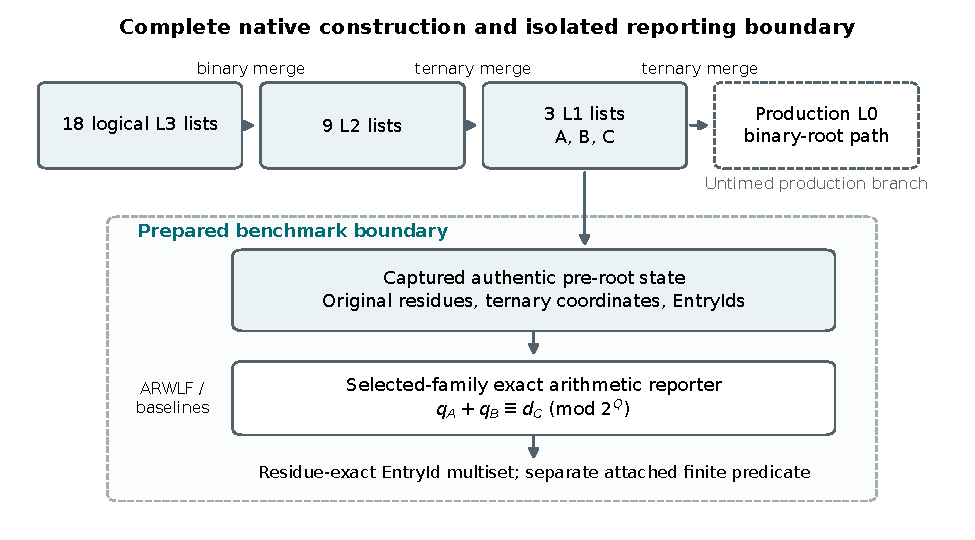
\includegraphics[width=\linewidth]{figures/topology.pdf}
\caption{Complete native TER list construction and the isolated prepared reporting boundary. The production binary-root branch is untimed and separate from the evaluated reporter. Captured native L1 lists provide arithmetic keys, stored residues, coordinate data and EntryIds; reported multisets do not construct a deduplicated L0 list or certify a solver solution.}
\Description{Flow diagram: 18 logical L3 lists merge to 9 L2 lists and then 3 L1 lists. A dashed, untimed production L0 branch is separate. A downward capture branch supplies an isolated prepared arithmetic reporter, which produces a residue-exact identity multiset and separate finite-predicate count.}
\label{fig:topology}
\end{figure}
\subsection{Exact quotient reduction}
Let $A,B,C$ be the three level-one lists. Each entry retains its original identity, vector, and residue. Suppose the inherited modulus is $2^{r_1}$ and each list has a fixed child target $c_A,c_B,c_C$. Valid prepared inputs satisfy $R_L\equiv c_L\pmod {2^{r_1}}$ for every entry in list $L$, and $T\equiv c_A+c_B+c_C\pmod {2^{r_1}}$. Define $Q=n-r_1$ and

\begin{equation*}
q_L=\frac{(R_L-c_L)\bmod 2^n}{2^{r_1}},\qquad
\tau=\frac{(T-c_A-c_B-c_C)\bmod 2^n}{2^{r_1}}.
\end{equation*}
The divisions are exact because of the inherited alignment. Quotients lie in $\mathbb Z/2^Q\mathbb Z$. With $d_C=\tau-q_C\pmod {2^Q}$, the root arithmetic becomes

\begin{equation*}
q_A+q_B\equiv d_C\pmod {2^Q}. \tag{1}
\end{equation*}
This reduction is target-aware. Shifting an unadjusted residue would not be an equivalent definition. Equation (1) follows by subtracting the three child targets from the original root congruence and dividing the resulting multiple of $2^{r_1}$.

\subsection{Family cells and retained key widths}
The low six quotient bits partition each source and target list into sixty-four families. For a source-family pair $(s,t)$, define $u=(s+t)\bmod 64$ and $\kappa=\lfloor(s+t)/64\rfloor$. The target family is $u$, and the family carry is $\kappa\in\{0,1\}$. There are 4,096 family cells, called microproblems below.

Let $F=\min(Q,64)$ and $W=F-6$. Within a cell, write the low-$F$ source and target keys as $s+64r_A$, $t+64r_B$, and $u+64r_Y$. Equation (1) then requires

\begin{equation*}
r_A+r_B+\kappa\equiv r_Y\pmod {2^W}. \tag{2}
\end{equation*}
If $Q>64$, the additional $Q-F$ bits must also match, with the carry out of the low-$F$ sum. They are retained separately. In the measured dimension-72 roots, $(r_1,Q,W)=(25,47,41)$; in the dimension-108 roots they are $(39,69,58)$. The latter therefore require five bits beyond the low sixty-four. No equality test may discard those bits.

Arithmetic equality is still only one level of acceptance. The common authority recomputes original residue equality modulo $2^n$ and applies an attached coordinate-closure and digit-count predicate. Original identities are preserved even when values coincide. Reporting arithmetic triples, satisfying that attached predicate, deduplicating parent vectors, and verifying a final binary witness are distinct operations. The principal exactness claim in this paper is full quotient and original-residue reporting, with the residue-exact identity multiset used as a differential gate.

The benchmark's attached structural predicate is a finite test-parent predicate, not the production binary-root predicate. Its negative, zero, and positive counts are $(2,56,14)$ at dimension 72 and $(2,86,20)$ at dimension 108; production roots require $(0,n/2,n/2)$. Authentic level-one vectors each have signed digit sum $n/6$, so a triple has signed digit sum $n/2$, whereas the attached predicate requires $n/6$. Authentic triples therefore cannot satisfy that predicate. Structural counters in the experiments are reported only with this meaning. This boundary does not change the arithmetic join being timed, but it rules out interpreting those counters as production-root certification.

\section{Baselines and the dense candidate problem}
\subsection{The tiled projected reporter}
The baseline, K2, evaluates source pairs in eight-by-eight tiles. It retains a nineteen-bit residual projection after the six family bits. For a projected sum $v$, its vector kernel tests a coarse bitmap whose bit represents a block of eight possible residual values. A passing lane is drained to scalar code, which recomputes $v$, performs exact membership in the nineteen-bit target bitmap, and expands every original target posting with that projected value. The shared sink then performs the remaining arithmetic and structural checks.

This is an exact arithmetic reporter when the downstream authorities are attached. Its early test is a necessary condition, not the final mathematical decision. The baseline is useful precisely because it preserves the original identity and multiplicity contract while exposing the cost of a short projection. Each target family uses a 64 KiB exact bitmap and an 8 KiB coarse bitmap. Across sixty-four families those two bitmap classes occupy 4.5 MiB, excluding postings, indexes, and authority data.

When large families populate the nineteen-bit residual space densely, the projected match rate can be substantial even though equality across forty-seven or sixty-nine quotient bits is rare. Every projected match invokes target-posting recovery and detailed downstream work. The bottleneck is not evidence that the vector kernel is poorly implemented; it is a consequence of the information retained by the early projection and the point at which discarded information is restored.

\subsection{A stronger full-width baseline}
K2-WIDE uses the same tile sweep and projected target directory, but compares the full retained residual and any extra high bits before calling the shared sink. It therefore tests a narrower hypothesis than the original baseline comparison: are gains explained solely by avoiding sink calls for low-width false candidates? K2-WIDE removes many such calls, yet still visits the target postings in each surviving projected group and retains the original coarse pair-processing path.

The wide residual addition is safe in the supported domain because $W\leq58$; two residuals and one carry fit in fifty-nine bits. The carry out of the $W$-bit result is added to the separately stored high quotient parts. Both K2-WIDE and ARWLF use this full-width comparison. Their reported acceptance therefore agrees at the same downstream authority level even though early candidate counters differ from K2's.

\subsection{The queued sparse reporter}
QUEUE-DENSE splits the nineteen-bit projection into a thirteen-bit position and a six-bit tag. For one source query it intersects translated target-position occupancy with source-position occupancy, compacts nonzero bitmap words, then resolves tags by a carry-aware cyclic rotation of sixty-four-bit tag masks. Group directories expand the matching relation to original postings. Full-width residue and structural decisions remain downstream.

The position space is fixed at 8,192 slots. The implementation's distinct-residual and hit capacity is 65,536 per relevant family; the dispatcher checks that capacity before admitting the reporter. The dimension-72 roots satisfy it, while the evaluated dimension-108 roots do not. QUEUE-DENSE is thus an informative legal alternative in the sparse regimes, rather than a missing timing entry that can be treated as zero runtime.

\section{Wide leaf filtering}
\subsection{Terminal partition and carry routing}
ARWLF partitions each family once, by the low thirteen residual bits. Let $H=2^{13}$. Write $r=\ell+Hm+\text{higher terms}$, where $\ell\in[0,H)$ is the leaf digit and $m$ contains the next $b=\min(32,W-13)$ bits. Each family retains leaf offsets, contiguous mids, and posting indexes back to the full keys and original identities. Target leaf $k$ stores four independent 256-bit occupancy maps, one for each possible mid byte.

For source leaves $i,j$ in a cell with carry $\kappa$, define

\begin{equation*}
k=(i+j+\kappa)\bmod H,\qquad
c=\left\lfloor\frac{i+j+\kappa}{H}\right\rfloor. \tag{3}
\end{equation*}
For fixed $k$ and $i$, the only compatible partner is $j=(k-i-\kappa)\bmod H$. The carry is zero when $i\leq k-\kappa$ and one otherwise. This makes leaf-sorted source rows two contiguous carry ranges. When $k=0$ and $\kappa=1$, the zero-carry range is empty; all rows belong to the carry-one range. Keeping this seam explicit avoids an unsigned-boundary shortcut that would change the mathematics.

The schedule visits only nonempty target leaves. A pair routed to an empty target leaf cannot satisfy Equation (2), so it needs no byte test. Within a nonempty target leaf, all assigned source rows run consecutively. The target summary stays fixed throughout that sweep.

\begin{figure}[htbp]
\centering
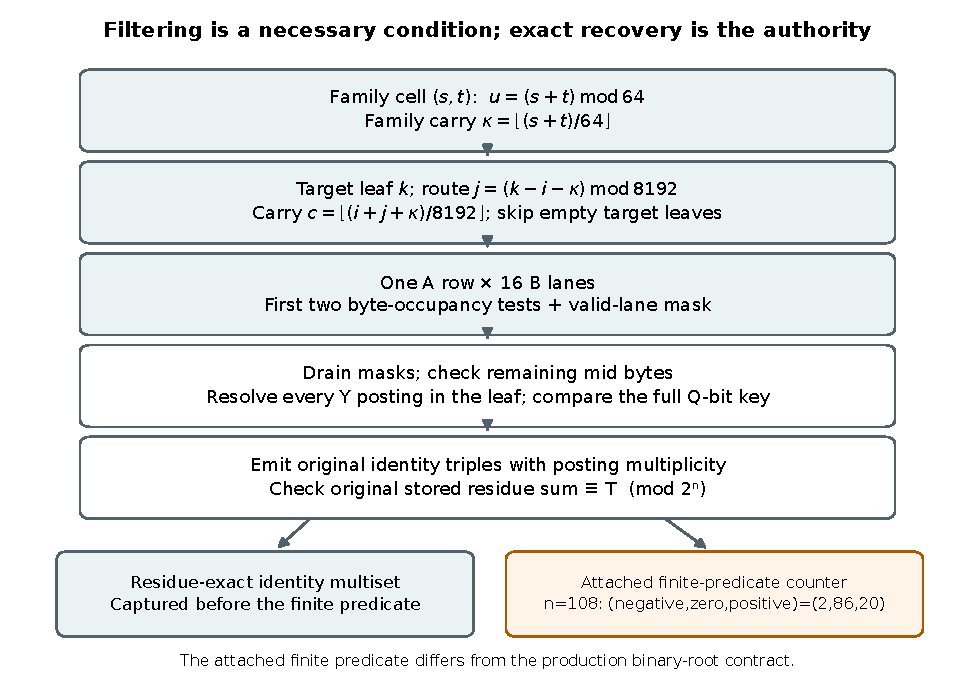
\includegraphics[width=\linewidth]{figures/pipeline.pdf}
\caption{ARWLF's routing, necessary byte predicates and exact survivor resolution. The arithmetic reporter retains every full quotient equality and original posting multiplicity. Residue-exact identities are collected before the attached FiniteSanity predicate, whose recorded n=108 counts (2,86,20) differ from the production binary-root counts (0,54,54).}
\Description{Five sequential boxes show family carry calculation, 13-bit leaf routing, one-row-by-16-lane byte tests, exact full-key resolution, and stored-residue checking. Output branches separately to the residue-exact multiset and the finite-predicate counter; n=108 finite counts are negative 2, zero 86, positive 20.}
\label{fig:pipeline}
\end{figure}
\subsection{Independent byte occupancy}
For target leaf $k$ and byte position $h$, define $B_{k,h}$ to contain every byte value occurring at position $h$ in a target mid. For a routed pair, compute

\begin{equation*}
m_*=(m_A+m_B+c)\bmod 2^b. \tag{4}
\end{equation*}
The pair passes the wide leaf filter only if every checked byte of $m_*$ belongs to the corresponding $B_{k,h}$. A true target equality contributes all of its bytes to those maps, so it cannot be rejected. The converse does not hold. Byte values may be present because of different target entries. ARWLF intentionally keeps these false positives and resolves them later.

The default checks all available mid bits: four bytes at $b=32$, and four chunks with a restricted last chunk at $b=28$. If a diagnostic configuration declares a smaller checked width, only complete bytes wholly inside that width are used; a partial last byte is safe when the entire available mid is declared, since the unused high bits are zero. The final full-key comparison always remains necessary. The reported timing campaign uses the default full mid width.

An elementary occupancy model explains why this test is attractive without making a distributional assumption part of correctness. Suppose a leaf contains $d$ independently sampled target mids, with $h$ independent uniform full bytes in each draw, and the query mid is independent of all target draws. Then

\begin{equation*}
\Pr[\text{byte filter passes}]=\left(1-\left(\frac{255}{256}\right)^d\right)^h. \tag{5}
\end{equation*}
For one byte, the absence probability is $(255/256)^d$. Under the stated model the target draws for distinct byte positions are independent, so the per-byte presence probabilities multiply. Equation (5) is an explanatory model, not a measured false-positive rate or a guarantee for TER data. Correlation, duplicates, partial bytes, and constructed targets can change the observed rate. In particular, increasing target occupancy makes the maps saturate and weakens rejection.

\subsection{One source row and sixteen lanes}
The optimized operation pairs one $A$ entry with sixteen $B$ entries in its compatible leaf. The low-sixteen-bit mids form one leaf-sorted dense array with sixteen global tail-padding entries. A short leaf load may also read entries from a neighboring leaf; a precomputed valid mask excludes every lane outside the current leaf. The $A$ preparation stores the two low-sixteen-bit addends for carry zero and carry one, each duplicated across the two sixteen-bit halves of a thirty-two-bit broadcast.

One AVX2 addition forms sixteen mid sums modulo $2^{16}$. Byte lookup tables represent the first two target occupancy maps in a shuffle-friendly layout. Lane-local byte shuffles retrieve membership bytes, bit tests identify missing values, and a byte movemask summarizes failures. The two byte failures for lane $i$ are combined; bit $2i$ of the resulting mask is set only if both bytes pass and the lane is valid. A row tentatively writes its source index and pass mask to contiguous pending scratch, advancing the logical length only when at least one lane survives.

The pending masks are drained outside the flat row loop. Full thirty-two-bit mids are reconstructed for surviving lanes, and any remaining byte chunks are checked there. Leaves containing more than sixteen $B$ entries receive additional sixteen-lane blocks in a separate overflow pass, with a valid mask on the final block. Consequently, the phrase sixteen-by-sixteen packet describes an occupancy accounting unit, not a machine instruction that computes 256 sums at once. The hardware operation is one row against sixteen lanes.

\subsection{Exact recovery and multiplicity}
Pairs surviving all byte maps are buffered for one target leaf. Each is compared with every target posting in that leaf. The resolver first checks the declared mid projection, then all $W$ residual bits, then the additional $Q-F$ high bits with the propagated carry. Only a full quotient match reaches the common sink.

The sink independently checks a low-thirty-two-bit quotient relation, recomputes equality of the original residue sum and root target modulo $2^n$, and applies the attached vector predicate described in Section 2.3. A residue-exact triple can fail that predicate. The residue-exact multiset used for differential comparison is captured before the structural decision; it is not a list of verified binary Subset Sum solutions. For constructed records, even consistency between coordinate data and stored residues is an additional property that these checks do not establish.

Every posting remains distinct. If equal-valued entries have different identities, the resolver enumerates their separate matches. The reporter performs no canonical-parent deduplication. This is necessary both for equivalence with the baselines and for charging output-heavy cases correctly.

\subsection{Semantic algorithm}
Algorithm 1 abstracts the row intrinsics while retaining the executed routing and authority semantics. VECTOR-BYTE-TEST returns precisely the valid lanes passing the first two byte maps; it makes no full-equality claim.

\noindent\begin{minipage}{\linewidth}
\begin{lstlisting}[basicstyle=\ttfamily\small,breaklines=true,columns=fullflexible,keepspaces=true]
Algorithm 1  ARWLF on a selected family cell
Prepare leaf partitions and target byte occupancy maps.
For each nonempty target leaf k in ascending order:
    Clear this leaf's survivor buffer.
    Split A rows into carry-zero and carry-one ranges.
    For each carry range:
        Clear pending row scratch for this range.
        For each source row a in that range:
            j <- (k - leaf(a) - family_carry) mod 8192
            mask <- VECTOR-BYTE-TEST(a, first 16 B_j lanes, carry)
            Record nonzero masks in pending row scratch.
        Drain pending masks using this range's carry and test remaining mid bytes.
    Sweep the additional B_j blocks for overflow leaves.
    For each surviving original source pair (a,b):
        For every target posting y in leaf k:
            If declared mid bits and all quotient bits match:
                Emit the original identity triple to the authority.
\end{lstlisting}
\end{minipage}
Preparation is lazy by family and cached within one backend call. The semantic algorithm assumes full target-leaf coverage and successful completion. Prefix probes and an aborted guarded execution do not constitute complete reporting.

\section{Correctness}
\textbf{Lemma 1 (unique compatible routing).} For a selected family cell, each source pair belongs to exactly one leaf relation in Equation (3). Any target satisfying Equation (2) belongs to that target leaf, with the stated carry.

\textbf{Proof.} Euclidean division of $i+j+\kappa$ by $H$ uniquely determines remainder $k$ and quotient $c$. Since $0\leq i,j<H$ and $\kappa\leq1$, the quotient is zero or one. Solving for $j$ gives $(k-i-\kappa)\bmod H$. If $k-i-\kappa\geq0$, no wrap is needed and $c=0$; otherwise the representative adds $H$ and $c=1$. This proves the two-range rule, including the empty zero-carry range at $k=0,\kappa=1$. Reducing Equation (2) modulo $H$ forces exactly this leaf relation.

\textbf{Lemma 2 (safe byte rejection).} Under valid preparation, the byte filter rejects no pair that participates in a full quotient match.

\textbf{Proof.} A full match implies Equation (2). After the leaf equality has been accounted for, the next $b$ bits are Equation (4). The matching target's mid therefore has every checked byte of $m_*$. Preparation sets each corresponding occupancy bit, so every checked membership test succeeds. Restricting the filter to complete declared byte chunks can only weaken rejection. The restricted final byte of a full-width mid is equal on both sides because its unused bits are zero.

\textbf{Lemma 3 (vector coverage).} The row and overflow sweeps evaluate every source pair routed to a visited target leaf, without allowing padding to become a survivor.

\textbf{Proof.} Leaf partitioning is a stable permutation of source postings. Every $A$ posting occurs in exactly one carry range for a given $k$. Its unique partner leaf is traversed in blocks of sixteen entries: the main block covers the first sixteen and overflow blocks cover the disjoint remainder. The lane-valid mask removes positions beyond the actual final block. The first two byte predicates operate on modular sixteen-bit sums, exactly the low sixteen bits of Equation (4). The survivor path reconstructs the wider sum before checking later bytes. Together these operations implement the scalar byte predicate for every actual assigned pair.

\textbf{Theorem 1 (exact quotient reporting and authority preservation).} Assume valid aligned prepared input, recoverable original postings and supported indexes, supported keys with $35\leq Q\leq69$, a reset output sink, full target-leaf coverage with work divisor one, successful allocation, and a completed ARWLF execution. Then, for every selected cell, ARWLF emits exactly the original identity triples satisfying Equation (1), with posting multiplicity preserved. When correctly populated residue and vector tables are attached, the sink identifies exactly the emitted subset satisfying original stored-residue equality and its attached closure and digit-count predicate.

\textbf{Proof.} A full quotient match has its unique compatible leaf by Lemma 1, and that leaf is nonempty. Lemmas 2 and 3 ensure that its pair survives to resolution. Resolution traverses every original target posting in the leaf, so the matching identity triple is considered. It compares all $W$ residual bits and, where present, the high quotient bits with the carry, hence emits the match. Conversely, emission requires those same equalities, which reconstruct Equation (1); no byte-only match is emitted. Posting indexes recover each original identity without coalescing equal values. The shared authority applies its exact predicates independently to every emitted triple, giving the final statement.

The theorem is conditional on successful full execution. A reduced prefix may return a completed prefix status yet omit undeclared leaves; an aborted or inapplicable call is not a negative result. When a guarded dispatcher retries another backend, it clears partial output before executing the fallback. Neither a completed empty selected-cell report nor exhaustion of a TER attempt proves global UNSAT.

\section{Cost and storage}
\subsection{Row work and occupancy}
Let $a_i,b_j,c_k$ be posting counts in the three leaf partitions of one family cell, and $K^+=\{k:c_k>0\}$. The logical source-pair mass is $P=|A_s||B_t|$. The routed mass requiring byte tests is

\begin{equation*}
P_+=\sum_{k\in K^+}\sum_i a_i b_{(k-i-\kappa)\bmod H}\leq P.
\end{equation*}
Pairs assigned to empty target leaves are removed by routing. They are still included in the reported total logical pair mass $P$, so nanoseconds per logical pair is an amortized accounting statistic, not the latency of an individual lane.

The main vector sweep executes $|K^+||A_s|$ rows, including rows whose partner slot is empty. The overflow contribution is

\begin{equation*}
R_{\rm over}=\sum_{k\in K^+}\sum_i a_i
\max\left(0,\left\lceil\frac{b_{(k-i-\kappa)\bmod H}}{16}\right\rceil-1\right).
\end{equation*}
Thus $R=|K^+||A_s|+R_{\rm over}$ is the number of physical sixteen-lane tests. In densely populated target families, $P_+$ approaches $P$ and much of each row is useful. Sparse partner leaves waste lanes, while the main-row traversal remains. Fixed vector width changes the constant cost of a covered pair; it does not make the dense pair term subquadratic.

The census also counts conceptual sixteen-by-sixteen packets over nonempty compatible leaf triples:

\begin{equation*}
\Pi=\sum_{k\in K^+}\sum_{i:b_j>0}
\left\lceil\frac{a_i}{16}\right\rceil
\left\lceil\frac{b_j}{16}\right\rceil. \tag{6}
\end{equation*}
Here $j=(k-i-\kappa)\bmod H$ and $L=P_+/\Pi$. For nonempty work, $1\leq L\leq256$. This occupancy measure predicts amortization, but is not itself a vector throughput measurement. The dispatcher uses a related estimate formed from per-family packet totals, with a conservative admission threshold. Observed $L$ in the plots comes from the exact census.

\subsection{Survivor and output work}
Let $S_k$ be the number of source pairs surviving all checked bytes for target leaf $k$, $V$ the number passing the first two bytes, and $E$ the number of full quotient triples emitted. On fixed-width hardware a useful implementation cost expression is

\begin{equation*}
T_{\rm work}=O\left(N+fH+R+B_{\rm over}+V+\sum_k S_kc_k+E\,C_{\rm auth}\right). \tag{7}
\end{equation*}
The overflow loop also incurs $B_{\rm over}=|K^+|\sum_j\max(\lceil b_j/16\rceil-1,0)$ block traversals, including blocks whose compatible $A$ leaf is empty. Here $N$ is the total posting count in touched families, $f$ their number, and $C_{\rm auth}$ the cost of one original-residue and attached-predicate check. The $V$ term accounts for draining initial masks and checking later bytes. The resolver term is explicit because each surviving pair scans every target posting in its leaf. For the favorable measured dense regime it is small relative to the pair sweep. In an adversarial single-leaf distribution with saturated byte maps, the resolver can take $\Theta(|A_s||B_t||Y_u|)$ work. The method therefore has no unconditional quadratic total-time bound for arbitrary reporting inputs.

An output-sensitive cost cannot be removed by filtering: every emitted identity triple must be recovered, and vector validation scales with the dimension. Equal-valued postings can multiply $E$ even when the number of distinct parent vectors is small. No complexity claim in this paper silently replaces posting multiplicity with unique-parent count.

\subsection{Memory}
Target summaries require $4\cdot256$ bits, or 128 bytes, per leaf. Allocating all 8,192 summaries uses 1 MiB per touched target family and at most 64 MiB for all sixty-four. Source partitions, row addends, lane slots, full keys, and the pending mask array add storage linear in their prepared entries plus fixed per-family leaf directories.

ARWLF avoids a complete table of all source-pair sums. It nevertheless stores the pairs surviving one target leaf, and that vector retains its capacity across leaves. With $S_{\max}=\max_k S_k$, its auxiliary storage is $O(N+fH+S_{\max})$, in addition to shared authority data and any retained outputs. $S_{\max}$ can be quadratic in source-family sizes. A small measured cache-size counter would not establish an unconditional linear-memory bound or a process peak bound.

\subsection{Adaptive selection}
The frozen dispatcher considers QUEUE-DENSE, ARWLF, and K2-WIDE. It checks the queued reporter's capacity, admits ARWLF only when its width and packet-amortization rules hold, and probes the legal candidates on a common selected subset. K2-WIDE probes a prefix of source blocks, while ARWLF probes a prefix of nonempty target leaves. Predictions scale preparation and sweep work separately. The smallest finite predicted time determines the backend; ties retain a fixed order.

A selected ARWLF run can be guarded against the runner-up's predicted break-even time per logical pair. After a sufficient prefix, an unfavorable estimate aborts it and the runner-up starts from cleared output. This is a practical heuristic, not a universal regret theorem. Probe overhead matters most when the selected problem is tiny, and the admission threshold can exclude profitable cases. Those effects are part of the results rather than hidden by reporting only the backend ultimately selected.

\section{Experimental design}
\subsection{Workloads and independent units}
The main campaign captures ten authentic pre-root states: six at dimension 108 and four at dimension 72. Three dimension-108 seeds, 0x1001, 0x2003, and 0x3007, are calibration roots that influenced development. Seeds 0x4001, 0x5003, and 0x6007 are campaign holdout roots captured after the preregistration was frozen. At dimension 72 there is one calibration anchor and three holdout roots, seeds 0x7201, 0x7203, and 0x7207. Original instance targets are planted; the term authentic describes the complete native list construction, not an unplanted random-target solver trial.

Each root receives a census of all 4,096 cells. An anchor cell is selected by a fixed deterministic shuffle. Additional cells are selected by preregistered strata in pair mass and packet occupancy. After the census but before timing, an amendment restricts dimension-108 strata to the four corners of the original grid, because those roots are internally nearly uniform and the full timing sweep is expensive. Dimension-72 roots retain the complete stratified selection. A corner that coincides with the anchor is not timed twice. This gives fourteen authentic dimension-108 calibration cells and fifteen holdout cells.

Cells from the same root share the input instance and list construction. They are not independent instance replications. Aggregate speedups are consequently accompanied by a root-block bootstrap. The three holdout roots are the independent holdout units; fifteen cells do not establish generalization to fifteen independently generated instances.

\subsection{Controlled geometry and target density}
Source thinning retains entries of $A_s$ and $B_t$ by a deterministic hash of root, cell, list tag, original identity, and thinning seed. It leaves keys and attached authority unchanged. Three thinning seeds are used per calibration root. Retention is selected by an untimed census bisection to reach requested occupancies from $L=1$ through $96$, with unreachable targets recorded explicitly. These are controlled reductions of dimension-108 source families, not authentic TER instances at smaller dimensions.

Target thinning retains only entries of $Y_u$ at fractions one-half, one-quarter, and one-eighth, with source families untouched. It isolates the effect of target occupancy and projected candidate recovery. Comparisons use the same transformed input for all backends. Neither transformation is included in the authentic headline.

\subsection{Machine, protocol, and timed boundary}
Measurements use an Intel Core Ultra 9 275HX, pinned to P-core logical CPU 23, on AC power with EcoQoS disabled. The program is C++20, compiled in MSVC Release mode; the recorded compiler identifier is 195136257. Optimization uses /O2 and /Ob2 with native AVX2 translation units. All backends execute single-threaded on identical prepared inputs.

Every case begins with an untimed exactness pass. The final protocol uses three warmup rounds and seven timed rounds; the discovery protocol uses one warmup and three timed rounds. Backend order rotates by round and reverses on odd rounds. Anchors, dimension-72 whole roots, and crossover confirmations use the final protocol. Strata and most thinning cases use discovery. The pooled authentic headline therefore combines these two declared protocols; the final-protocol anchors are also reported separately.

Timing includes the backend call, its lazy internal preparation, survivor resolution, shared sink processing, and dispatcher probes where applicable. Snapshot loading, common dataset conversion, full-key and common-index preparation, exactness passes, census, and post-call witness sorting are outside the prepared-backend comparison. A repeated pass rebuilds ARWLF's per-call cache; it does not reuse an uncharged persistent leaf index. Prepared-backend timings do not include complete TER list generation.

A CPU sentinel records machine conditions at process boundaries and during the campaign. Some resumed source-thinning points have slower sentinel readings; their matched ratios are retained. No accepted sample is recorded off the pinned core. This is one processor and one implementation toolchain, not a hardware-portability study.

\subsection{Exactness gates and statistics}
For each timed case, sorted residue-exact identity multisets agree with the K2 reference. Intermediate width-count and hash gates compare ARWLF with K2-WIDE and K2's narrower checks; a separately computed census agrees with counted geometry. Structural counts, identity hashes, directory misses, and residual mismatches are checked at their declared levels. Synthetic tests add whole-value modular brute-force comparisons and scalar/vector filter comparisons, including carry seams and overflow leaves.

All 221 completed campaign cases pass the recorded gates. Three source-thinning targets are unreachable, leaving 224 declared cases. The accepted timing set contains 3,220 samples; nine rows from incomplete cases are excluded from summaries and retained as partial evidence. All authentic and thinned campaign cases have zero full-quotient matches, residue-exact triples, and structural outputs. Agreement at those output gates is therefore supplemented by intermediate counts, independent bounded tests, and the constructed positive experiments below. Zero-output agreement alone would not validate recovery.

For case $i$, speedup is the median K2 time divided by the median candidate time. Multiplicative results aggregate as $G=\exp(\frac1m\sum_i\log S_i)$. Percentile bootstrap intervals use 10,000 resamples with fixed seed 0xB007. The root-block bootstrap resamples whole root clusters and retains their cells together. With only three roots per dimension-108 role, these intervals characterize the observed design and are not broad population guarantees. Dispatcher regret is its median time divided by the minimum median among applicable exact reporters, including K2.

\subsection{Constructed outputs and full prepared roots}
A separate experiment appends controlled target records to one authentic cell. For a selected authentic source pair, a constructed target has the full key and residue needed for arithmetic equality, and coordinate data chosen so the summed parent passes the attached finite test-parent predicate. A decoy condition appends the same number of target records without valid final outputs. The original source families and authentic target records are retained.

These appended records have ternary coordinate data but are not established members of the native level-one TER sets. Their stored residues and coordinate completions are assigned separately; equality with the coordinate dot product of the original weights is not established. The completion targets the attached finite test-parent predicate, not the binary production root. They test arithmetic filtering and identity recovery under prescribed output loads, and do not create authentic solver solutions. The completed repeated subset available for this paper comprises one calibration root and three samples per case. Other scheduled roots are not included as if their runs had finished.

The complete dimension-108 prepared-root experiment uses seed 0x1001, all 4,096 cells, and one constructed positive target. ARWLF and the dispatcher run in one call to retain their within-call family caches. Each available completed pass is a single measurement, without the campaign warmup and repeated-round protocol. The baseline run is checkpointed by target family and is incomplete at the evidence cutoff. Its partial time is not extrapolated into a measured whole-root speedup.

AI coding assistants were used during the implementation and manuscript workflow. For this article, Codex assisted source interpretation, literature synthesis, statistical recomputation, analysis scripts, figure generation, and drafting; the supplied development session records Claude-assisted campaign and solver work. Numerical results originate from retained native-run artifacts, and deterministic scripts compute the reported tables from those artifacts. The correctness argument states explicit hypotheses independently of any assistant's assertions.

\section{Results}
\subsection{Dense authentic microproblems}
Table 1 reports the six final-protocol anchors in seconds, allowing the ratios to be checked directly. The source-pair mass is approximately $6.1\cdot10^9$ for seed 0x1001 and $1.2\cdot10^{10}$ for the other roots. ARWLF takes 0.842 to 1.679 seconds per anchor; K2 takes 44.558 to 131.159 seconds. The largest ratio occurs because K2 is slow on the 0x2003 anchor. It is retained, but it does not define the headline by itself.

\begin{table}[htbp]
\caption{Final-protocol medians for six authentic dimension-108 anchor cells (seconds).}
\label{tab:anchors}
\small
\begin{tabularx}{\linewidth}{@{}>{\raggedright\arraybackslash}X>{\centering\arraybackslash}X>{\centering\arraybackslash}X>{\centering\arraybackslash}X>{\centering\arraybackslash}X>{\centering\arraybackslash}X>{\centering\arraybackslash}X@{}}
\toprule
\textbf{Seed} & \textbf{Role} & \textbf{L} & \textbf{K2} & \textbf{K2-WIDE} & \textbf{ARWLF} & \textbf{Dispatch} \\
\midrule
0x1001 & calibration & 78.44 & 44.5583 & 27.1931 & 0.8424 & 0.8642 \\
0x2003 & calibration & 126.26 & 131.1588 & 54.5698 & 1.6794 & 1.7017 \\
0x3007 & calibration & 127.33 & 86.3898 & 54.5793 & 1.6376 & 1.6537 \\
0x4001 & holdout & 125.94 & 83.9879 & 53.2772 & 1.6578 & 1.6739 \\
0x5003 & holdout & 126.13 & 85.6578 & 54.2728 & 1.6549 & 1.6717 \\
0x6007 & holdout & 125.56 & 84.4173 & 52.3676 & 1.6107 & 1.6260 \\
\bottomrule
\end{tabularx}
\par\smallskip\footnotesize Three warmup rounds and seven timed rounds per cell; each value is a median. All rows cover one selected cell, not a whole root. QUEUE-DENSE is capacity-inapplicable. The 0x2003 K2 median has IQR 91.0567–145.7907 s; that row is retained.
\end{table}
Across all declared authentic cells, the calibration geometric mean is 53.0875 and the holdout mean is 52.8933 (Table 2). Their root-block 95 percent bootstrap intervals are 48.17 to 57.61 and 51.81 to 53.81. The similar holdout gain supports the dense operating regime on the three additional roots. It does not remove dependence among cells or establish results at other dimensions.

\begin{table}[htbp]
\caption{Geometric-mean speedups on authentic dimension-108 cells, with the final-protocol subset kept separate.}
\label{tab:aggregates}
\small
\begin{tabularx}{\linewidth}{@{}>{\raggedright\arraybackslash}X>{\centering\arraybackslash}X>{\centering\arraybackslash}X>{\centering\arraybackslash}X>{\centering\arraybackslash}X>{\centering\arraybackslash}X@{}}
\toprule
\textbf{Subset} & \textbf{Roots / cells} & \textbf{K2 / ARWLF} & \textbf{Wide / ARWLF} & \textbf{K2 / dispatch} & \textbf{95\% CI: K2 / ARWLF} \\
\midrule
Pooled cells, calibration & 3 / 14 & 53.0875 & 32.7769 & 52.3649 & [48.17, 57.61] \\
Pooled cells, holdout & 3 / 15 & 52.8933 & 32.4378 & 52.3819 & [51.81, 53.81] \\
Final anchors, calibration & 3 / 3 & 60.1774 & 32.6977 & 59.2128 & [52.75, 78.10] \\
Final anchors, holdout & 3 / 3 & 51.6060 & 32.4806 & 51.1069 & [50.66, 52.41] \\
\bottomrule
\end{tabularx}
\par\smallskip\footnotesize Pooled estimates weight cells equally and combine declared discovery/final protocols. Intervals resample entire roots as blocks (10,000 percentile draws, seed 0xB007); only three independent roots occur per role. Equal-root calibration sensitivity gives 52.7449, 32.7335, and 52.0020 for the three ratios; holdout equal-root estimates coincide with pooled estimates. Final anchors have one cell per root.
\end{table}
K2-WIDE improves on K2 by about 1.62 to 1.63 in the pooled sets. ARWLF remains faster than K2-WIDE by geometric means of 32.78 on calibration cells and 32.44 on holdout cells. Moving full-width comparison before the shared sink is beneficial, but it does not explain the full ARWLF result. ARWLF also changes the inexpensive pair test and suppresses target-posting visits before the exact resolver.

The authentic dimension-108 census has $L$ near 78 for the first calibration root and near 126 for the remaining roots. Within a root, cell pair mass and occupancy vary little. Figure 3 shows all twenty-nine individual speedups rather than only their means. The spread includes slow baseline cases and a holdout ARWLF timing outlier; no case is removed for being inconvenient.

\begin{figure}[htbp]
\centering
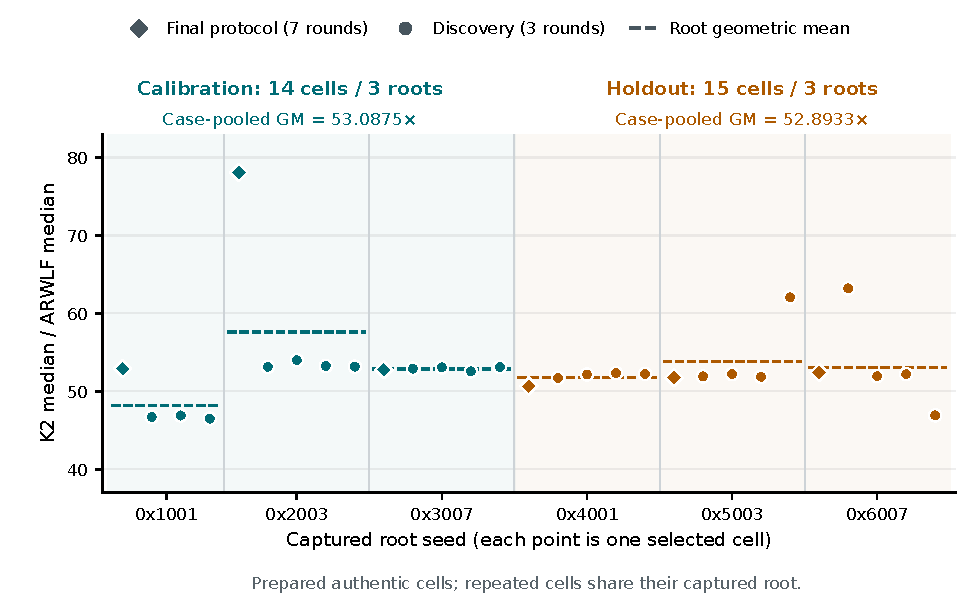
\includegraphics[width=\linewidth]{figures/dense.pdf}
\caption{All 29 declared authentic dimension-108 cell speedups, grouped by captured root and calibration role. Diamonds use the final protocol (seven timed rounds) and circles discovery (three); dashed segments show each root's geometric mean. Aggregate labels are case-pooled geometric means. Repeated cells share their root and are not independent instances.}
\Description{Scatterplot of all 29 K2/ARWLF median ratios across six root-seed groups. Calibration points are teal; holdout points orange. Diamonds indicate seven-round final anchors and circles three-round discovery cases. Per-root geometric means are dashed. Most ratios lie near 47 to 54; the 0x2003 final anchor is about 78, with holdout discovery points near 62 to 63 and one near 47.}
\label{fig:dense}
\end{figure}
\subsection{Occupancy crossover}
Controlled source thinning changes the amortization without changing the quotient width or target family. At $L=1$, ARWLF loses: the rows and preparation are poorly amortized. At $L=2$, it wins on all three calibration roots, with discovery-protocol speedups over K2 ranging from 4.4 to 6.7 and gains over the fastest applicable rival of about 2.6 to 3.3. Final-protocol confirmations at the two bracket points reproduce a loss at one and a gain of approximately 2.7 to 3.4 over the fastest rival at two.

\begin{figure}[htbp]
\centering
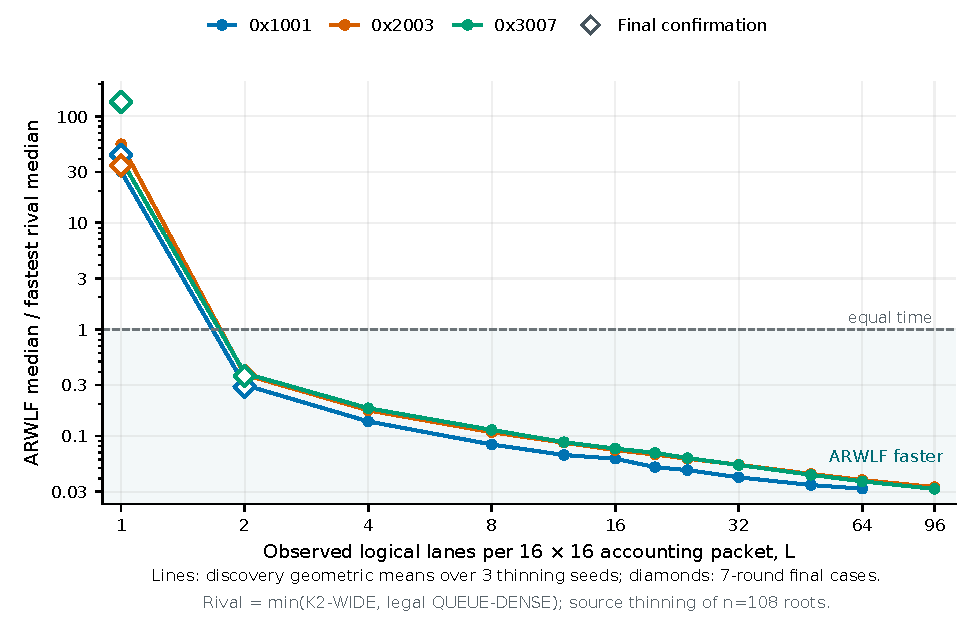
\includegraphics[width=\linewidth]{figures/crossover.pdf}
\caption{Controlled source-thinning crossover for three calibration dimension-108 roots. Discovery lines use geometric means over three thinning seeds; plotted L is their geometric-mean observed census occupancy. Open diamonds are separate final-protocol confirmations using seed 0xA11CE001. Ratios below one favor ARWLF. Lines connect measured points, not a fitted or universal threshold. Target L=96 is unreachable for root 0x1001.}
\Description{Log-log plot of ARWLF/rival time ratio against observed packet occupancy L for three source-thinned roots. Discovery averages over three thinning seeds are colored connected circles; final confirmations are open diamonds. Ratios exceed one at L=1 and fall below one near L=2, approaching about 0.03 at the densest tested controls.}
\label{fig:crossover}
\end{figure}
As source occupancy increases, ARWLF's advantage grows. This is a finite-regime crossover observed under this target geometry, rather than a universal threshold for arbitrary key distributions. Equation (7) explains the dependence: sparse blocks spend vector work on few real lanes, while dense blocks amortize the same row operation. Target selectivity, duplicated keys, and output load can move the crossover independently of $L$.

\subsection{Target-density ablation}
Figure 5 holds source pairs fixed and thins only the target family. Reducing target density accelerates K2 substantially, as fewer projected matches require posting expansion and downstream work. ARWLF also becomes faster, but its decrease is smaller. For seed 0x1001, the median K2 time falls from 44.56 seconds at full density to 8.31 seconds at one-eighth density, while ARWLF falls from 0.842 to 0.621 seconds. The corresponding speedup falls from 52.89 to 13.38.

\begin{figure}[htbp]
\centering
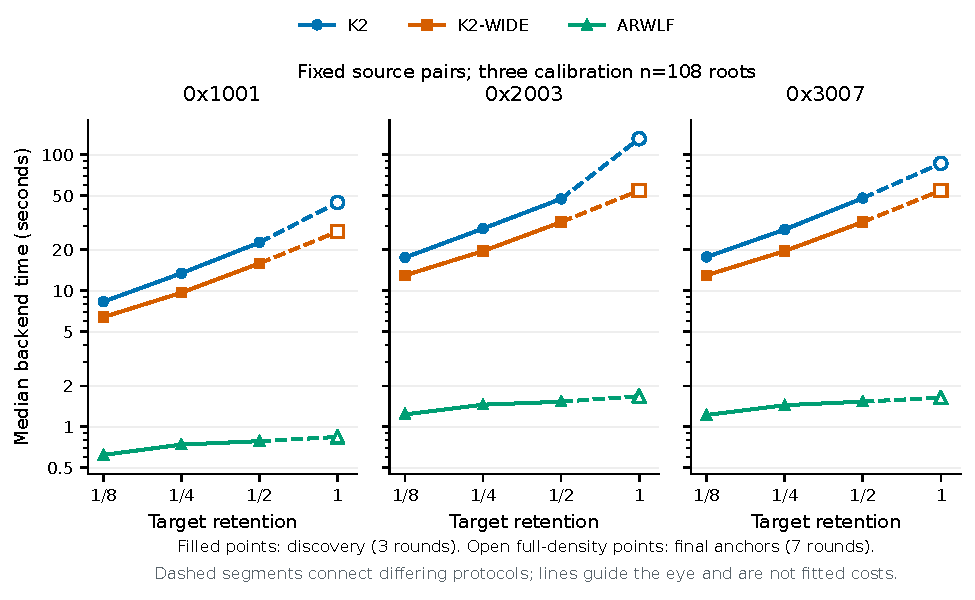
\includegraphics[width=\linewidth]{figures/target.pdf}
\caption{Absolute median times under target-only thinning with fixed source-pair mass on three calibration roots. Filled points use discovery (one warmup, three timed rounds); open full-density references use final anchors (three warmups, seven timed rounds). Dashed connections mark the protocol change. Target thinning is a controlled sensitivity experiment, not a smaller-dimension authentic benchmark.}
\Description{Three side-by-side panels show absolute median times for K2, K2-WIDE and ARWLF as target retention increases from one-eighth to one. K2 and K2-WIDE become much slower with denser targets, while ARWLF changes more modestly. Open full-density points use seven-round final anchors; filled thinned points use three-round discovery cases, with dashed segments separating the protocols.}
\label{fig:target}
\end{figure}
The result supports a mechanism involving both cheap physical pair processing and early suppression of projected candidates. It does not isolate an exact causal percentage for either. Removing target entries changes byte occupancy, posting lists, and the set of nonempty leaves together. The experiment is consequently a controlled sensitivity study, not a decomposition into independently additive instruction costs.

\subsection{Sparse complete roots and dispatcher behavior}
The dimension-72 roots have $L$ near one. Table 3 reports complete prepared-root timings under the final repeated protocol. QUEUE-DENSE is faster than K2 by factors of 1.21 to 1.84; ARWLF is slower than K2 by factors of approximately 3.4 to 7.0. The dispatcher runs QUEUE-DENSE on all four roots, with regret between 1.039 and 1.140.

\begin{table}[htbp]
\caption{Complete authentic dimension-72 prepared-root medians (milliseconds), covering all 4,096 cells.}
\label{tab:sparse}
\small
\begin{tabularx}{\linewidth}{@{}>{\raggedright\arraybackslash}X>{\centering\arraybackslash}X>{\centering\arraybackslash}X>{\centering\arraybackslash}X>{\centering\arraybackslash}X>{\centering\arraybackslash}X>{\centering\arraybackslash}X@{}}
\toprule
\textbf{Root} & \textbf{K2} & \textbf{K2-WIDE} & \textbf{QUEUE-DENSE} & \textbf{ARWLF} & \textbf{Dispatch} & \textbf{Regret} \\
\midrule
anchor (cal.) & 301.499 & 298.367 & 167.555 & 1137.442 & 178.176 & 1.0634 \\
0x7201 (hold.) & 327.703 & 317.924 & 269.858 & 2300.027 & 307.724 & 1.1403 \\
0x7203 (hold.) & 545.324 & 544.682 & 298.074 & 1846.978 & 309.589 & 1.0386 \\
0x7207 (hold.) & 551.480 & 556.351 & 299.240 & 2002.560 & 315.252 & 1.0535 \\
\bottomrule
\end{tabularx}
\par\smallskip\footnotesize Final protocol: three warmup and seven timed rounds. QUEUE-DENSE wins all four rows and the dispatcher runs it in every sample. Regret divides dispatcher median by the fastest legal reporter median, including K2. No end-to-end list-generation cost is included.
\end{table}
On all twenty-nine authentic dimension-108 cells, the dispatcher runs ARWLF. Its median regret is 1.010, its 95th percentile is 1.020, and its maximum is 1.026. This is favorable measured selection behavior in the dense regime. It coexists with two clear failures elsewhere. On tiny dimension-72 cells the fixed probe cost dominates roughly 0.1 ms of useful work, producing regret as high as 172.9. On source-thinned dimension-108 cases with observed occupancy from two through sixteen, the packet admission rule excludes ARWLF even when it is several times faster than the alternatives. At occupancy sixteen, maximum regret is 17.6.

The frozen dispatcher is therefore useful at the evaluated large-root scopes, but cannot be described as universally regret-bounded. Backend capability, admission policy, prediction quality, and probing cost must be evaluated separately. This paper reports the policy as measured rather than retrospectively changing the threshold to make the curve look better.

\subsection{Constructed positive outputs}
Table 4 reports the completed one-root constructed-output experiment. Each point has one warmup and three matched timed samples. At each appended count, the planted case and its decoy twin have the same target-list growth. The comparison exposes output and target-density effects jointly; it is not an authentic TER scaling series.

\begin{table}[htbp]
\caption{Constructed target augmentation on authentic source families of calibration root 0x1001: medians in seconds.}
\label{tab:positive}
\small
\begin{tabularx}{\linewidth}{@{}>{\raggedright\arraybackslash}X>{\centering\arraybackslash}X>{\centering\arraybackslash}X>{\centering\arraybackslash}X>{\centering\arraybackslash}X>{\centering\arraybackslash}X>{\centering\arraybackslash}X@{}}
\toprule
\textbf{Appended M} & \textbf{Condition} & \textbf{Residue-exact} & \textbf{K2} & \textbf{K2-WIDE} & \textbf{ARWLF} & \textbf{Dispatch} \\
\midrule
100 & positive & 100 & 46.1093 & 27.7730 & 0.9115 & 0.9283 \\
100 & decoy & 0 & 45.2586 & 27.7191 & 0.9103 & 0.9230 \\
1,000 & positive & 1,000 & 78.9186 & 30.8078 & 1.0205 & 1.0547 \\
1,000 & decoy & 0 & 73.0600 & 27.6073 & 0.8851 & 0.9043 \\
10,000 & positive & 10,000 & 51.6717 & 29.1376 & 0.9143 & 0.9291 \\
10,000 & decoy & 0 & 59.6852 & 29.2994 & 0.9071 & 0.9128 \\
100,000 & positive & 100,000 & 80.6972 & 44.5106 & 1.1462 & 1.1775 \\
100,000 & decoy & 0 & 72.2938 & 44.3863 & 1.0401 & 1.0643 \\
1,000,000 & positive & 1,000,000 & 248.8130 & 101.0825 & 20.4859 & 20.6871 \\
1,000,000 & decoy & 0 & 263.4709 & 105.1932 & 19.4581 & 19.6438 \\
\bottomrule
\end{tabularx}
\par\smallskip\footnotesize Every case uses one warmup and three timed rounds. Residue-exact counts also equal the attached finite-predicate counts in these records: M for positives and zero for decoys. That predicate has (negative, zero, positive) = (2,86,20), not the production binary-root distribution. Constructed coordinates and residues are assigned separately; original-weight consistency and native L1 membership are unestablished. Only one root has completed repeated evidence.
\end{table}
All prescribed planted identities are recovered and satisfy the attached finite predicate, while decoys produce no residue-exact or structural outputs. As the target leaves grow, their byte maps become less selective and the survivor resolver has more target postings to scan. At one million appended entries, ARWLF takes 20.486 seconds in the positive condition and 19.458 seconds in the decoy condition. Much of the slowdown is therefore present without emitted outputs and is consistent with target/filter saturation; it cannot be charged entirely to per-output emission. These measurements demonstrate positive arithmetic recovery on the constructed contract. They neither establish the natural distribution of TER solutions nor validate a complete solver on the added targets.

\subsection{A complete dimension-108 prepared root}
The completed ARWLF pass covers 25,189,929,333,072 logical pairs across all 4,096 cells and reports the prescribed single identity triple. Its backend time is 3,575.458 seconds, or 59.591 minutes. The dispatcher pass selects ARWLF, reports the identical residue-exact triple and structural count, and takes 3,557.074 seconds, or 59.285 minutes. Measured process peaks are 3,278.5 and 3,278.6 MiB. Table 5 separates setup and backend time.

\begin{table}[htbp]
\caption{Single complete dimension-108 prepared-root passes, with measured setup separated from backend time.}
\label{tab:whole}
\small
\begin{tabularx}{\linewidth}{@{}>{\raggedright\arraybackslash}X>{\centering\arraybackslash}X>{\centering\arraybackslash}X@{}}
\toprule
\textbf{Component} & \textbf{ARWLF} & \textbf{Dispatch (ran ARWLF)} \\
\midrule
Snapshot load (s) & 7.5778 & 7.6819 \\
Target construction (s) & 0.2707 & 0.3100 \\
Full-key preparation (s) & 0.2586 & 0.2770 \\
Root-index preparation (s) & 0.1354 & 0.1565 \\
Census (s) & 0.0272 & 0.0295 \\
Total setup (s) & 8.2697 & 8.4549 \\
Backend (s) & 3575.4581 & 3557.0744 \\
Process peak (MiB) & 3278.5 & 3278.6 \\
\bottomrule
\end{tabularx}
\par\smallskip\footnotesize Each pass covers 4,096 cells and 25,189,929,333,072 logical pairs with one constructed target and the same residue-exact EntryId triple. There are no warmup/repeat-based dispersion estimates. Capture and earlier snapshot I/O are excluded. Peaks include common authorities/setup, not just a backend index. K2 is incomplete at the frozen cutoff; no whole-root speedup is inferred.
\end{table}
The slightly shorter dispatcher pass is not evidence that probing improves the kernel; these are separate single passes under different machine conditions. ARWLF's amortized time is approximately 0.142 ns per logical pair, including its within-call preparation and authority work. This normalization represents many-lane processing, not subnanosecond scalar execution.

The first ARWLF pass is unguarded, and the protocol records background activity and Windows page compression. No repeated-run dispersion estimate is available for these completed passes. They establish that this prepared full-root scope completes and handles the constructed output on the measured machine. A completed baseline whole-root comparison, a representative multi-root whole-root campaign, and an end-to-end TER solve remain outside the measured result.

\section{Relation to prior work}
\subsection{Subset Sum representations and exact algorithms}
Horowitz and Sahni split an instance into two parts and compare enumerated subset sums, establishing the classical meet-in-the-middle baseline \cite{hs1974}. Schroeppel and Shamir preserve the half-exponent time scale while reducing storage by generating ordered pair sums from four smaller lists \cite{ss1981}. These are general exact approaches. ARWLF neither replaces their worst-case algorithms nor implements a Schroeppel-Shamir recovery structure; it optimizes a three-list merge arising inside a specific representation construction.

Howgrave-Graham and Joux introduce multiple representations to exploit hard random knapsacks \cite{hgj2010}. Becker, Coron, and Joux extend the technique using signed entries and filtering, and analyze a heuristic $2^{0.291n}$ time regime \cite{bcj2011}. Their explicit treatment of pre-filter intermediate lists is particularly relevant here: the cost of rejected arithmetic candidates cannot be inferred from the final valid list. Bonnetain, Bricout, Schrottenloher, and Shen analyze improved classical and quantum representation algorithms \cite{bbss2020}. Li's later TER construction uses ternary merges and a depth-three topology, with a heuristic random density-one time bound $2^{0.2400n}$ \cite{li2025}. The finite-width reporter in this paper operates within such list geometry; it does not prove or improve those heuristic exponents.

Nederlof and Węgrzycki use representations and orthogonal vectors to improve Schroeppel and Shamir's space exponent in a Monte Carlo algorithm for worst-case instances, while retaining its half-exponent time scale \cite{nw2021}. Chen, Jin, Randolph, and Servedio obtain a randomized polynomial-factor improvement over the meet-in-the-middle time bound for worst-case Subset Sum using bit packing and representation methods \cite{cjrs2023}. Their word width grows with the instance encoding; a fixed sixteen-lane instruction alone would not establish that asymptotic improvement. These results demonstrate that word-level computation and representation ideas can yield theoretical improvements when supported by an asymptotic analysis. ARWLF's fixed sixteen-lane row sweep is instead a measured constant-factor engineering result, with explicit survivor costs and no claimed improvement of the general exact bound.

\subsection{Packed reporting and machine-oriented joins}
Baran, Demaine, and Pătraşcu give subquadratic 3SUM algorithms in computational models that exploit packing and word-level parallelism \cite{bdp2008}. Barba and coauthors study algebraic generalizations of 3SUM under real-RAM and algebraic decision-tree models, distinguishing decision from output-sensitive reporting \cite{barba2017}. A modular three-list equality resembles these settings arithmetically, but the measured TER workload also carries original-entry multiplicity and vector constraints. More fundamentally, ARWLF continues to cover dense source-pair mass at fixed vector width. A small amortized cost per pair is not a subquadratic pair count. The prior 3SUM result is a useful boundary for terminology, not a claimed consequence of this implementation.

Late materialization is established in column-oriented databases: predicates can be evaluated before assembling full tuples \cite{abadi2007}. Radix partitioning and hardware-conscious hash joins are also established techniques \cite{balkesen2013}. SIMD database work studies efficient predicate evaluation, gathers, scatters, and lane management \cite{polychroniou2015}. Earlier SIMD scans evaluate predicates directly on compressed values and expose the cost of expanding scan masks into output positions \cite{willhalm2009}. ARWLF shares the broader principle of keeping hot representations compact and postponing expensive identity work. Its specific formulation combines power-of-two carries, terminal residual leaves, independent byte occupancy, a target-leaf row schedule, and exact TER downstream authority. The contribution is that integration and its measured operating regime, not the invention of radix partitioning, bitmap membership, SIMD, or late materialization.

\section{Discussion and limits}
The evidence supports a simple design lesson: when a short projection creates a flood of candidates, moving high-information necessary conditions ahead of recovery can matter more than reducing the apparent count of valid outputs. K2-WIDE shows that early full-width rejection alone helps; ARWLF shows that a much cheaper filter and a different row organization can improve further. Target thinning then connects the gain to the baseline's projected-candidate sensitivity. Together these comparisons explain the architectural result without assigning the entire speedup to AVX2.

The dense advantage has a boundary. Sparse leaves waste lanes and expose preparation cost. Duplicated or highly correlated target mids can saturate independent byte maps, enlarge the survivor buffer, and increase leaf scans. Constructed output stress exercises that path, but remains a one-root controlled experiment. Memory and time should therefore be predicted from entries, row occupancy, survivor counts, target-leaf sizes, and output multiplicity together. A single list-size threshold is insufficient.

The holdout design is stronger than reporting a single favorable anchor, but modest in independent-instance count. Its fifteen holdout cells derive from three roots on one processor. The root-block intervals respect that clustering, yet cannot establish processor-independent performance or all-density behavior. Additional machines and complete repeated-root comparisons would answer distinct questions, rather than merely add more samples of the same cells.

The evaluated backend is also separate from production solving. Preparation captures authentic native lists, and the arithmetic authority checks their stored modular residues. The benchmark's finite test-parent predicate differs from the binary production root and is incompatible with authentic root digit sums. A full integration must use the production predicate, preserve complete list-generation and failure semantics, recover and deduplicate parents as required, and independently recompute any claimed binary witness against the original instance. None of those end-to-end costs can be inferred from a prepared-cell ratio. The complete prepared-root pass establishes arithmetic-reporting feasibility at that boundary, while the incomplete baseline comparison remains an open measurement rather than an estimated result.

\section{Conclusion}
ARWLF routes TER root pairs through fixed terminal leaves and uses inexpensive byte occupancy before exact identity recovery. The routing and filter preserve every full quotient match, including carries beyond sixty-four bits, and the original-residue check retains the modular arithmetic contract. The measured dense dimension-108 regime yields a 52.9-fold holdout gain over the tiled baseline and a 32.4-fold gain over its full-width strengthening. Sparse roots favor another reporter, and controlled thinning exposes both the crossover and the dispatcher's limits. The result is an exact, finite-size improvement in prepared arithmetic root reporting whose pair, survivor, output, and memory costs remain explicit; binary-root certification requires a separate production integration.

\section{Data and code availability}
The implementation and campaign artifacts are associated with the subset-sum-ter-fft research project. The manuscript supplement contains deterministic table and figure scripts, input-file hashes, and a record of the exact evidence cutoff. Snapshot identity metadata are retained, but the large snapshot byte files are not part of the manuscript source bundle. Reproducing native timings requires the recorded snapshots, compatible build, and machine protocol; recomputing the reported tables requires the retained raw campaign rows. The large snapshots and native source are retained in the project repository; access to those materials is required to repeat native timings.

\section{Acknowledgments}
Codex assisted preparation of the manuscript, including source checking, literature synthesis, deterministic statistical analysis scripts, figures, and prose. The continued development session also records Claude assistance.

\clearpage
\begin{thebibliography}{99}
\bibitem{abadi2007}
Daniel J. Abadi, Daniel S. Myers, David J. DeWitt and Samuel R. Madden. 2007. Materialization Strategies in a Column-Oriented DBMS. 2007 IEEE 23rd International Conference on Data Engineering, 466–475.
\url{https://doi.org/10.1109/ICDE.2007.367892}.
\bibitem{balkesen2013}
C. Balkesen, J. Teubner, G. Alonso and M. T. Ozsu. 2013. Main-memory hash joins on multi-core CPUs: Tuning to the underlying hardware. 2013 IEEE 29th International Conference on Data Engineering (ICDE), 362–373.
\url{https://doi.org/10.1109/ICDE.2013.6544839}.
\bibitem{bdp2008}
Ilya Baran, Erik D. Demaine and Mihai Pǎtraşcu. 2008. Subquadratic Algorithms for 3SUM. Algorithmica 50(4), 584–596.
\url{https://doi.org/10.1007/s00453-007-9036-3}.
\bibitem{barba2017}
Luis Barba, Jean Cardinal, John Iacono, Stefan Langerman, Aurélien Ooms and Noam Solomon. 2017. Subquadratic Algorithms for Algebraic Generalizations of 3SUM. 33rd International Symposium on Computational Geometry (SoCG 2017) 77, 13:1–13:15.
\url{https://doi.org/10.4230/LIPIcs.SoCG.2017.13}.
\bibitem{bcj2011}
Anja Becker, Jean-Sébastien Coron and Antoine Joux. 2011. Improved Generic Algorithms for Hard Knapsacks. Advances in Cryptology -- EUROCRYPT 2011 6632, 364–385.
\url{https://doi.org/10.1007/978-3-642-20465-4_21}.
\bibitem{bbss2020}
Xavier Bonnetain, Rémi Bricout, André Schrottenloher and Yixin Shen. 2020. Improved Classical and Quantum Algorithms for Subset-Sum. Advances in Cryptology -- ASIACRYPT 2020 12492, 633–666.
\url{https://doi.org/10.1007/978-3-030-64834-3_22}.
\bibitem{cjrs2023}
Xi Chen, Yaonan Jin, Tim Randolph and Rocco A. Servedio. 2023. Subset Sum in Time $2^{n/2}/\operatorname{poly}(n)$. Approximation, Randomization, and Combinatorial Optimization. Algorithms and Techniques (APPROX/RANDOM 2023) 275, 39:1–39:18.
\url{https://doi.org/10.4230/LIPIcs.APPROX/RANDOM.2023.39}.
\bibitem{hs1974}
Ellis Horowitz and Sartaj Sahni. 1974. Computing Partitions with Applications to the Knapsack Problem. Journal of the ACM 21(2), 277–292.
\url{https://doi.org/10.1145/321812.321823}.
\bibitem{hgj2010}
Nick Howgrave-Graham and Antoine Joux. 2010. New Generic Algorithms for Hard Knapsacks. Advances in Cryptology -- EUROCRYPT 2010 6110, 235–256.
\url{https://doi.org/10.1007/978-3-642-13190-5_12}.
\bibitem{li2025}
Yang Li. 2025. From Subset-Sum to Decoding: Improved Classical and Quantum Algorithms via Ternary Representation Technique. Information 16(10), 887.
\url{https://doi.org/10.3390/info16100887}.
\bibitem{nw2021}
Jesper Nederlof and Karol Węgrzycki. 2021. Improving Schroeppel and Shamir’s algorithm for subset sum via orthogonal vectors. Proceedings of the 53rd Annual ACM SIGACT Symposium on Theory of Computing, 1670–1683.
\url{https://doi.org/10.1145/3406325.3451024}.
\bibitem{polychroniou2015}
Orestis Polychroniou, Arun Raghavan and Kenneth A. Ross. 2015. Rethinking SIMD Vectorization for In-Memory Databases. Proceedings of the 2015 ACM SIGMOD International Conference on Management of Data, 1493–1508.
\url{https://doi.org/10.1145/2723372.2747645}.
\bibitem{ss1981}
Richard Schroeppel and Adi Shamir. 1981. A $T=O(2^{n/2})$, $S=O(2^{n/4})$ Algorithm for Certain NP-Complete Problems. SIAM Journal on Computing 10(3), 456–464.
\url{https://doi.org/10.1137/0210033}.
\bibitem{willhalm2009}
Thomas Willhalm, Nicolae Popovici, Yazan Boshmaf, Hasso Plattner, Alexander Zeier and Jan Schaffner. 2009. SIMD-Scan: Ultra Fast in-Memory Table Scan using on-Chip Vector Processing Units. Proceedings of the VLDB Endowment 2(1), 385–394.
\url{https://doi.org/10.14778/1687627.1687671}.
\end{thebibliography}
\clearpage
\appendix
\section{Reproducibility details}
The source basis includes the SHA-256-pinned frozen root backends at revision \texttt{8e9fe7fd\allowbreak{}da447088\allowbreak{}738b5e68\allowbreak{}2ba6aea4\allowbreak{}cf83a121} and local campaign additions for constructed targets and complete-root replay. The regime campaign build record preserves its earlier dirty-tree freeze separately; a Git commit alone is not a substitute for its source manifest. Supplementary hashes identify every numerical input used to construct the article. The long-running baseline is read only at the recorded cutoff, and incomplete rows are excluded from complete-run comparisons.

The principal result tables are computed from the accepted timed rows, grouped by root, case, and backend. Their medians agree with the retained case summaries. Regime status, protocol, source transformation, and calibration role remain part of every group key. Ratios use within-case matched inputs. Complete-root single-pass times are not pooled with repeated-cell medians, and constructed positives are not pooled with authentic output-free cases.

\begin{table}[htbp]
\caption{Measurement protocols and completed case counts, preserving workload and scope boundaries.}
\label{tab:protocols}
\small
\begin{tabularx}{\linewidth}{@{}>{\raggedright\arraybackslash}X>{\centering\arraybackslash}X>{\centering\arraybackslash}X>{\centering\arraybackslash}X>{\centering\arraybackslash}X@{}}
\toprule
\textbf{Dataset / phase} & \textbf{Cases} & \textbf{Warmups} & \textbf{Timed rounds} & \textbf{Protocol} \\
\midrule
n=108, anchor & 6 & 3 & 7 & final \\
n=108, stratified-corners & 23 & 1 & 3 & discovery \\
n=72, whole & 4 & 3 & 7 & final \\
n=72, anchor & 4 & 3 & 7 & final \\
n=72, stratified & 64 & 1 & 3 & discovery \\
n=108, thin-qx & 105 & 1 & 3 & discovery \\
n=108, confirm & 6 & 3 & 7 & final \\
n=108, thin-y & 9 & 1 & 3 & discovery \\
Positive / decoy augmentation & 10 & 1 & 3 & discovery \\
n=108 complete-root passes & 2 & 0 & 1 & single pass \\
Unreachable source-thinning cases & 3 & — & — & no timing \\
\bottomrule
\end{tabularx}
\par\smallskip\footnotesize The first eight rows sum to 221 completed regime cases. Nine orphan timings from one interrupted attempt remain outside those complete-case groups. All 10 roots are censused at all 4,096 cells; census is not timing. Cases from one root share an independent input instance. Three unreachable rows are statuses, not omitted failures or timed points.
\end{table}
The supplemental analysis verifies all 221 completed case groups and retains nine incomplete timing rows outside the aggregate set. Figures use exact observed occupancy and the declared target retention, not a dimension inferred from thinning. Appendix B provides additional absolute timings for the controls, while the ledger identifies source and derivation for every principal claim.

\section{Additional control timings}
\begin{table}[htbp]
\caption{Target-density ablation medians (seconds), with full-density anchor protocol stated explicitly.}
\label{tab:target_detail}
\small
\begin{tabularx}{\linewidth}{@{}>{\raggedright\arraybackslash}X>{\centering\arraybackslash}X>{\centering\arraybackslash}X>{\centering\arraybackslash}X>{\centering\arraybackslash}X>{\centering\arraybackslash}X@{}}
\toprule
\textbf{Seed} & \textbf{Target retention} & \textbf{Protocol} & \textbf{K2} & \textbf{K2-WIDE} & \textbf{ARWLF} \\
\midrule
0x1001 & 1 & final & 44.5583 & 27.1931 & 0.8424 \\
0x1001 & 1/2 & discovery & 22.6460 & 15.9057 & 0.7848 \\
0x1001 & 1/4 & discovery & 13.4524 & 9.6796 & 0.7401 \\
0x1001 & 1/8 & discovery & 8.3117 & 6.4016 & 0.6214 \\
0x2003 & 1 & final & 131.1588 & 54.5698 & 1.6794 \\
0x2003 & 1/2 & discovery & 47.3672 & 31.9722 & 1.5288 \\
0x2003 & 1/4 & discovery & 28.6618 & 19.5796 & 1.4543 \\
0x2003 & 1/8 & discovery & 17.5418 & 12.9889 & 1.2339 \\
0x3007 & 1 & final & 86.3898 & 54.5793 & 1.6376 \\
0x3007 & 1/2 & discovery & 48.0082 & 31.9832 & 1.5320 \\
0x3007 & 1/4 & discovery & 28.1909 & 19.5958 & 1.4422 \\
0x3007 & 1/8 & discovery & 17.7154 & 13.0133 & 1.2211 \\
\bottomrule
\end{tabularx}
\par\smallskip\footnotesize Source pair mass is fixed within each root. Full-density references use three warmups/seven timed rounds; thinned cases use one/three, seed 0xA11CE001. Target thinning changes occupancy/filter selectivity and posting recovery, while observed packet occupancy L is nearly unchanged. This is a controlled sensitivity study, not an isolated causal instruction-cost decomposition.
\end{table}
\begin{table}[htbp]
\caption{Final-protocol confirmations of the source-thinning crossover bracket.}
\label{tab:crossover_confirm}
\small
\begin{tabularx}{\linewidth}{@{}>{\raggedright\arraybackslash}X>{\centering\arraybackslash}X>{\centering\arraybackslash}X>{\centering\arraybackslash}X>{\centering\arraybackslash}X>{\centering\arraybackslash}X@{}}
\toprule
\textbf{Seed} & \textbf{Observed L} & \textbf{K2-WIDE (ms)} & \textbf{ARWLF (ms)} & \textbf{ARWLF / rival} & \textbf{Dispatch regret} \\
\midrule
0x1001 & 1.0000 & 0.0395 & 1.7126 & 43.3570 & 2.2203 \\
0x1001 & 1.9998 & 155.4762 & 45.1552 & 0.2904 & 3.6530 \\
0x2003 & 1.0000 & 0.0614 & 2.1208 & 34.5407 & 2.1270 \\
0x2003 & 1.9999 & 169.3821 & 62.0819 & 0.3665 & 2.8158 \\
0x3007 & 1.0000 & 0.0105 & 1.4286 & 136.0571 & 4.1429 \\
0x3007 & 1.9999 & 181.6719 & 66.3434 & 0.3652 & 2.8233 \\
\bottomrule
\end{tabularx}
\par\smallskip\footnotesize Three warmups/seven timed rounds, thinning seed 0xA11CE001. Rival = min(K2-WIDE, legal QUEUE-DENSE); QUEUE-DENSE is capacity-inapplicable here. Ratios below one favor ARWLF. The dispatcher runs K2-WIDE in all six cases; it misses the measured ARWLF gain near L=2. The two tested points bracket rather than identify an exact universal threshold.
\end{table}
The target-density table keeps the source pair mass fixed within each root. The crossover table uses only the final-protocol confirmations; discovery sweep curves are displayed separately in Figure 4. These controls address different mechanisms and are not combined into an additional authentic benchmark headline.

\end{document}